% PrivacyGNN technical deep-dive guide
% Build from this directory:
%   pdflatex PROJECT_TECHNICAL_DEEP_DIVE.tex
%   pdflatex PROJECT_TECHNICAL_DEEP_DIVE.tex
\documentclass[10pt,a4paper]{article}
\usepackage[margin=0.72in]{geometry}
\usepackage[T1]{fontenc}
\usepackage{lmodern}
\usepackage{microtype}
\usepackage{xcolor}
\usepackage{hyperref}
\usepackage{booktabs}
\usepackage{array}
\usepackage{longtable}
\usepackage{amsmath}
\usepackage{tikz}
\usetikzlibrary{arrows.meta,positioning,calc,shapes.geometric,fit}

\hypersetup{
  colorlinks=true,
  linkcolor=blue!55!black,
  urlcolor=blue!55!black,
  citecolor=blue!55!black
}

\definecolor{ink}{HTML}{0F172A}
\definecolor{muted}{HTML}{475569}
\definecolor{teal}{HTML}{0F766E}
\definecolor{bluebox}{HTML}{EFF6FF}
\definecolor{greenbox}{HTML}{ECFDF5}
\definecolor{orangebox}{HTML}{FFF7ED}
\definecolor{redbox}{HTML}{FEF2F2}
\definecolor{graybox}{HTML}{F8FAFC}

\setlength{\parskip}{0.45em}
\setlength{\parindent}{0pt}
\renewcommand{\arraystretch}{1.22}

\makeatletter
\def\@listi{\leftmargin\leftmargini \topsep 3pt \parsep 2pt \itemsep 2pt}
\makeatother

\newcommand{\code}[1]{\texttt{\detokenize{#1}}}
\newcommand{\file}[1]{\texttt{\detokenize{#1}}}
\newcommand{\keyterm}[1]{\textbf{\textcolor{teal}{#1}}}
\newcolumntype{L}[1]{>{\raggedright\arraybackslash}p{#1}}

\title{\textbf{PrivacyGNN: Complete Technical Deep Dive}\\
\large Every major concept, file, method, dependency, output, and limitation}
\author{Prepared for Krish Sharma}
\date{\today}

\begin{document}
\maketitle

\begin{abstract}
This document is a deep technical guide to the \textbf{PrivacyGNN} project. It explains the research problem, graph-learning background, membership inference attacks, model architectures, defenses, experiment grid, code modules, output files, visualization scripts, paper-generation tools, dependencies, testing status, and known limitations. It is written so you can learn the project from first principles and then map each concept directly to the codebase.
\end{abstract}

\tableofcontents
\newpage

%==============================================================================
\section{Executive Summary}
%==============================================================================

\textbf{PrivacyGNN} studies whether graph neural networks leak membership information: can an attacker infer whether a node was part of the training set by looking at the model's prediction probabilities? The codebase is a reproducible experiment framework for node-classification privacy experiments.

The central workflow is:
\begin{enumerate}
  \item Load or generate a graph dataset.
  \item Split nodes into train and test members.
  \item Train a model: feature-only baseline or GNN.
  \item Optionally apply a lightweight defense.
  \item Use prediction probabilities to run membership inference attacks.
  \item Save utility, privacy, calibration, and graph-structure metrics.
  \item Aggregate results, test defense effects, bootstrap uncertainty, and generate figures.
\end{enumerate}

\textbf{Important reality check for this checkout:}
\begin{itemize}
  \item Current results contain \textbf{560 rows}: 8 datasets, 4 models, 6 defenses for GNNs, 5 seeds.
  \item \file{lira_attack.py} is a placeholder returning chance-level scores.
  \item \file{ogb_loader.py} and \file{graph_minibatch.py} are stubs; large-graph OGB/Reddit/minibatch/DP-SGD paths are not active in this snapshot.
  \item There is no dedicated unit-test directory or pytest suite discovered. Validation is currently through reproducible runs, CSV outputs, plotting scripts, and statistical summaries.
\end{itemize}

%==============================================================================
\section{Project at a Glance}
%==============================================================================

\begin{center}
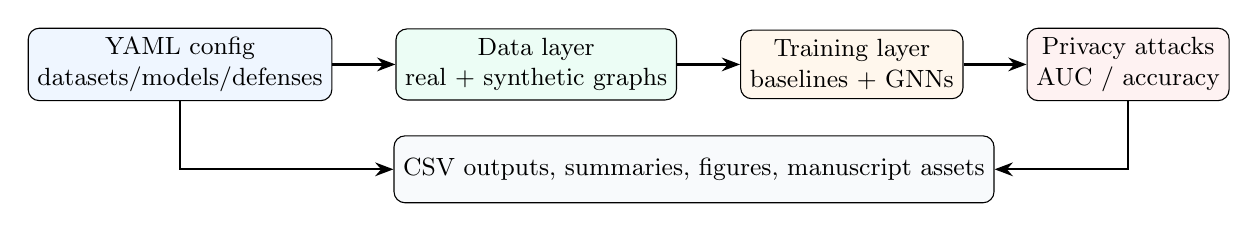
\begin{tikzpicture}[
  font=\small,
  box/.style={draw,rounded corners,align=center,minimum width=2.3cm,minimum height=0.85cm},
  arr/.style={-{Stealth},thick}
]
\node[box,fill=bluebox] (cfg) {YAML config\\datasets/models/defenses};
\node[box,fill=greenbox,right=0.8cm of cfg] (data) {Data layer\\real + synthetic graphs};
\node[box,fill=orangebox,right=0.8cm of data] (train) {Training layer\\baselines + GNNs};
\node[box,fill=redbox,right=0.8cm of train] (att) {Privacy attacks\\AUC / accuracy};
\node[box,fill=graybox,below=0.9cm of $(data)!0.5!(train)$] (out) {CSV outputs, summaries, figures, manuscript assets};
\draw[arr] (cfg) -- (data);
\draw[arr] (data) -- (train);
\draw[arr] (train) -- (att);
\draw[arr] (att.south) |- (out.east);
\draw[arr] (cfg.south) |- (out.west);
\end{tikzpicture}
\end{center}

The project is mostly \textbf{Python}. It also uses \textbf{YAML} for configuration, \textbf{Bash} for orchestration, \textbf{LaTeX} and \textbf{ReportLab} for PDFs, \textbf{Markdown} for analysis notes, and \textbf{CSV} files for experiment outputs.

%==============================================================================
\section{Repository Structure}
%==============================================================================

The active repository root is \file{privacy-gnn/}. The table below explains every important source artifact.

\begin{longtable}{@{}L{0.28\textwidth}L{0.66\textwidth}@{}}
\toprule
\textbf{File / folder} & \textbf{Role in the project}\\
\midrule
\endhead
\file{README.md} & Human-facing overview, setup commands, project structure, research questions, and notes about newer extensions versus paper configuration.\\
\file{requirements.txt} & Python dependency list: PyTorch, PyTorch Geometric, OGB, Opacus, NumPy, sklearn, pandas, scipy, matplotlib, seaborn, ReportLab, PyYAML, and plotting helpers.\\
\file{config.py} & Central configuration loader. Reads YAML, provides defaults, converts defense dictionaries into tuples, builds the experiment grid, and creates output directories.\\
\file{experiment_config.yaml} & Main large config. Uses 10 seeds, includes LiRA placeholder and DP-SGD/large graph settings, though large-graph execution is stubbed here.\\
\file{experiment_config_paper.yaml} & Paper-aligned grid: 5 seeds, Cora, Citeseer, six synthetics, confidence/threshold/shadow attacks, no LiRA or DP-SGD.\\
\file{data.py} & Dataset loading and graph utilities: Cora/Citeseer loading, synthetic graph generation, train/test resplitting, homophily, density, and random edge dropping.\\
\file{models.py} & Two GNN architectures: two-layer GCN and two-layer GraphSAGE. Baselines are not here; they are sklearn models in \file{experiment.py}.\\
\file{training.py} & Full-batch GNN training loop with DropEdge, label smoothing, early stopping, and edge sparsification support.\\
\file{attacks.py} & Core membership inference attacks and calibration: feature extraction, confidence attack, threshold attack, shadow attack, and ECE.\\
\file{experiment.py} & The single-run engine. Loads one dataset/model/defense/seed combination, trains target and shadow models, runs attacks, and returns a flat metrics row.\\
\file{stats_utils.py} & Statistical utilities: paired t-tests defense-vs-none, LiRA t-test wrapper, bootstrap confidence intervals over seeds.\\
\file{run_final.py} & Main runner. Builds full experiment grid, iterates over runs, writes all results, summary, significance, LiRA significance, and bootstrap CSVs.\\
\file{generate_figures.py} & Publication-style six-figure generator from \file{results/all_results.csv}; includes citation fallbacks and synthetic plots.\\
\file{generate_basic_figures.py} & Simpler four-figure synthetic visualization script from \file{summary.csv}.\\
\file{generate_final_visuals.py} & Polished visual suite for final presentation/poster, outputting to \file{../Final Visuals}.\\
\file{generate_poster_visuals.py} & Larger poster-ready visual suite: pipeline, heatmaps, privacy-utility plots, defense rankings, significance maps, calibration plots, and summary table.\\
\file{fix_figures.py} & Patch script for improved versions of Figure 2 and Figure 4, using \file{adjustText} for labels.\\
\file{ogb_loader.py} & Stub. \code{MINIBATCH_DATASETS} is empty and \code{load_large_benchmark} raises \code{NotImplementedError}.\\
\file{graph_minibatch.py} & Stub. Minibatch training, minibatch inference, and DP-SGD minibatch training all raise \code{NotImplementedError}.\\
\file{lira_attack.py} & Placeholder. \code{lira_gaussian_auc} returns \code{(0.5, 0.5)}.\\
\file{run_everything_final.sh} & Bash script that runs \file{run_final.py} and then \file{generate_figures.py}.\\
\file{RESULTS_ANALYSIS.md} & Human-written interpretation of synthetic results and research questions.\\
\file{paper/ieee_privacy_gnn.tex} & Main IEEE-style manuscript source.\\
\file{paper/build_manuscript.py} & ReportLab script that creates a static workshop-style \file{manuscript.pdf}. Some claims in this script should be checked against current code/results before reuse.\\
\file{paper/build_project_slides.py} & PowerPoint generation script using \file{python-pptx}. Produces a designed project overview deck.\\
\file{paper/literature_review.md} & Literature notes supporting the paper framing.\\
\file{results/*.csv} & Experiment outputs: per-run rows, summaries, significance tests, bootstrap CIs, and partial checkpoint.\\
\file{data/} & Downloaded PyG datasets and raw Planetoid files.\\
\file{docs/} & Learning PDFs generated for you, including this technical guide.\\
\bottomrule
\end{longtable}

%==============================================================================
\section{Languages, File Types, and Tooling}
%==============================================================================

\begin{longtable}{@{}L{0.18\textwidth}L{0.22\textwidth}L{0.54\textwidth}@{}}
\toprule
\textbf{Type} & \textbf{Where} & \textbf{Why it is used}\\
\midrule
\endhead
Python & \file{*.py} & Core experiments, model definitions, training, attacks, statistics, figures, manuscript/deck builders.\\
YAML & \file{experiment_config*.yaml} & Reproducible experiment definitions without editing source code.\\
Bash & \file{run_everything_final.sh} & One-command orchestration for full run plus figures.\\
CSV & \file{results/*.csv} & Durable tabular output, easy to analyze with pandas/spreadsheets.\\
LaTeX & \file{paper/*.tex}, \file{docs/*.tex} & Academic paper and guide PDFs.\\
Markdown & \file{README.md}, \file{RESULTS_ANALYSIS.md}, \file{paper/*.md} & Human-readable documentation and interpretation.\\
PowerPoint & \file{paper/build_project_slides.py} output & Presentation deck generation.\\
PNG/PDF figures & \file{figures/}, \file{../Final Visuals/} & Publication/poster/presentation visuals.\\
\bottomrule
\end{longtable}

%==============================================================================
\section{Dependencies and Libraries}
%==============================================================================

\begin{longtable}{@{}L{0.22\textwidth}L{0.72\textwidth}@{}}
\toprule
\textbf{Library} & \textbf{Purpose in this project}\\
\midrule
\endhead
\code{torch} & Tensor computation, neural network modules, optimization, softmax/logits, GNN training loops.\\
\code{torch-geometric} & Graph data object \code{Data}, Planetoid dataset loading, GCNConv, SAGEConv.\\
\code{ogb} & Listed for future large benchmark support, but current loader is stubbed.\\
\code{opacus} & Listed for DP-SGD privacy accounting, but current DP path is stubbed.\\
\code{numpy} & Random seeds, synthetic data generation, feature extraction, bootstrap sampling.\\
\code{scikit-learn} & Logistic regression, MLP baseline, attack classifiers, metrics.\\
\code{pandas} & CSV reading/writing, groupby aggregation, pivot tables for figures/statistics.\\
\code{scipy} & Paired t-tests through \code{scipy.stats}.\\
\code{matplotlib} & All generated figures.\\
\code{seaborn} & Heatmaps and visual style in publication figures.\\
\code{PyYAML} & Parse experiment configuration files.\\
\code{reportlab} & Programmatic PDF manuscript creation in \file{paper/build_manuscript.py}.\\
\code{adjustText} & Improved label placement in \file{fix_figures.py}.\\
\code{tqdm} & Listed dependency, not central in the current code paths.\\
\bottomrule
\end{longtable}

%==============================================================================
\section{Research Concepts You Need to Understand}
%==============================================================================

\subsection{Graph Node Classification}

The basic supervised task is node classification. Each node has:
\begin{itemize}
  \item feature vector \(x_i\),
  \item label \(y_i\),
  \item graph neighbors through \(\texttt{edge\_index}\),
  \item membership in train or test masks.
\end{itemize}

The model predicts a class distribution \(p(y \mid x_i, G)\). For baselines, \(G\) is ignored. For GNNs, \(G\) is essential because features are mixed through message passing.

\subsection{Membership Inference}

A membership inference attack asks:
\[
\text{Given model output for node } i,\quad \text{was } i \text{ in the training set?}
\]
In this project:
\begin{itemize}
  \item train-mask nodes are treated as \textbf{members},
  \item test-mask nodes are treated as \textbf{non-members},
  \item attack AUC near 0.5 means random guessing,
  \item attack AUC above 0.5 means membership leakage.
\end{itemize}

\subsection{Graph Homophily}

Homophily is computed in \file{data.py} as:
\[
\text{homophily} =
\frac{\#\{(u,v)\in E: y_u = y_v\}}{\#E}.
\]
High homophily means connected nodes usually share labels. Low homophily means edges often connect different labels.

\subsection{Graph Density}

Density is computed as:
\[
\text{density} =
\frac{\text{undirected edges}}{n(n-1)/2}.
\]
Sparse graphs have fewer neighbor messages; dense graphs have more smoothing and more structural signal.

%==============================================================================
\section{Data Layer in Detail}
%==============================================================================

\subsection{\texttt{data.py}: Citation Datasets}

\file{load_citation(name, data_dir)} uses \code{torch_geometric.datasets.Planetoid} to load Cora or Citeseer. It returns:
\[
(\texttt{data},\ \texttt{num\_classes},\ \texttt{num\_features})
\]
where \code{data} contains \code{x}, \code{edge_index}, \code{y}, and masks. If the default Planetoid URL fails, the function temporarily swaps \code{Planetoid.url} to a mirror URL.

\subsection{\texttt{data.py}: Synthetic Graph Generator}

\code{make_synthetic(n=400, nf=50, nc=5, homo="high", dens="medium", seed=42)} is one of the project's most important methods. It creates controlled graph regimes:
\begin{itemize}
  \item \(n=400\) nodes by default.
  \item \(nf=50\) features per node.
  \item \(nc=5\) classes.
  \item Labels are random class IDs.
  \item Class centers are Gaussian vectors.
  \item Node features are class center plus Gaussian noise.
  \item Density controls how many edges are sampled.
  \item Homophily controls same-label versus different-label edge fraction.
  \item Train/test split is 50/50.
\end{itemize}

\begin{center}
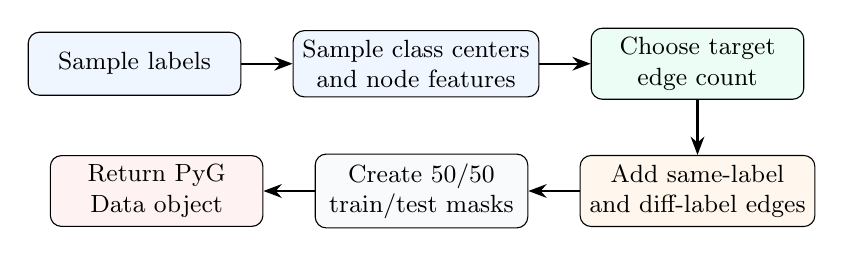
\begin{tikzpicture}[
  font=\small,
  box/.style={draw,rounded corners,align=center,minimum width=2.7cm,minimum height=0.8cm},
  arr/.style={-{Stealth},thick}
]
\node[box,fill=bluebox] (labels) {Sample labels};
\node[box,fill=bluebox,right=0.65cm of labels] (features) {Sample class centers\\and node features};
\node[box,fill=greenbox,right=0.65cm of features] (edgecount) {Choose target\\edge count};
\node[box,fill=orangebox,below=0.7cm of edgecount] (edges) {Add same-label\\and diff-label edges};
\node[box,fill=graybox,left=0.65cm of edges] (masks) {Create 50/50\\train/test masks};
\node[box,fill=redbox,left=0.65cm of masks] (data) {Return PyG\\Data object};
\draw[arr] (labels) -- (features);
\draw[arr] (features) -- (edgecount);
\draw[arr] (edgecount) -- (edges);
\draw[arr] (edges) -- (masks);
\draw[arr] (masks) -- (data);
\end{tikzpicture}
\end{center}

\subsection{Resplitting and Reproducibility}

\code{resplit(data, seed)} clones a graph and creates a fresh 50/50 train/test split. This means different seeds change which nodes are members and non-members. This is critical for paired comparisons across defenses.

\subsection{Edge Dropping}

\code{drop_edges(edge_index, rate)} randomly keeps each edge with probability \(1-\text{rate}\). It is used by:
\begin{itemize}
  \item DropEdge during training,
  \item edge sparsification before training,
  \item explicit edge preprocessing in \file{experiment.py} for minibatch/DP paths.
\end{itemize}

%==============================================================================
\section{Model Layer}
%==============================================================================

\subsection{Feature-only Baselines}

The baselines are defined inside \file{experiment.py}, not \file{models.py}:
\begin{itemize}
  \item \code{LogisticRegression(max_iter=1000)}
  \item \code{MLPClassifier(hidden_layer_sizes=(64, 32), max_iter=200)}
\end{itemize}
Both consume \code{data.x.numpy()} and ignore \code{edge_index}. They are important controls: they tell you how much privacy leakage comes from features and classifier confidence alone.

\subsection{GCN}

\file{models.py} defines:
\[
\text{GCNConv}(d_{\text{in}}, 64) \rightarrow \text{ReLU} \rightarrow \text{Dropout}(0.5) \rightarrow \text{GCNConv}(64, C)
\]
GCN uses graph convolution, where each layer aggregates information from neighbors using normalized adjacency. It is usually strong when homophily is high.

\subsection{GraphSAGE}

GraphSAGE follows the same two-layer layout, but uses \code{SAGEConv}. It aggregates neighbor features differently and is often more robust in inductive or noisy graph settings.

\subsection{Why Two GNNs Matter}

GCN and GraphSAGE are both message-passing models, but they do not behave identically. The result analysis notes that GCN can leak more in low-homophily sparse settings, while GraphSAGE often stays closer to random attack AUC.

%==============================================================================
\section{Training Layer and Defenses}
%==============================================================================

\file{training.py} is the full-batch GNN trainer. It takes a model, a PyG \code{Data} object, and training options.

\subsection{Base Optimization}

The base training loop:
\begin{enumerate}
  \item Move data/model to device.
  \item Create Adam optimizer.
  \item Optionally sparsify edges once.
  \item For each epoch:
    \begin{enumerate}
      \item optionally DropEdge for this epoch,
      \item forward pass,
      \item compute loss on \code{train_mask},
      \item backpropagate,
      \item optimizer step,
      \item optionally early-stop.
    \end{enumerate}
\end{enumerate}

\subsection{Defense Methods}

\begin{longtable}{@{}L{0.22\textwidth}L{0.24\textwidth}L{0.48\textwidth}@{}}
\toprule
\textbf{Defense} & \textbf{Where applied} & \textbf{Technical behavior}\\
\midrule
\endhead
\code{none} & Training/prediction baseline & No modification. Used as the reference for significance tests.\\
\code{dropedge} & Training-time & Drops random edges each epoch. In config, default rate is 0.3.\\
\code{label_smoothing} & Loss function & Replaces one-hot targets with softened class distributions. Config alpha is 0.1.\\
\code{early_stopping} & Training control & Tracks loss improvement and restores best state if patience expires. Config patience is 15.\\
\code{confidence_masking} & Post-prediction & Keeps top-\(k\) class probabilities and renormalizes. Config top\_k is 2.\\
\code{edge_sparsification} & Pre-training graph & Removes a fraction of edges once before training. Config rate is 0.2.\\
\code{dp_sgd} & Stub path & Config exists, but actual minibatch DP function is not implemented in this checkout.\\
\bottomrule
\end{longtable}

\subsection{Important Implementation Detail}

Confidence masking is not part of model training. In \file{experiment.py}, it is applied after probabilities are produced:
\[
p_i \leftarrow \text{keep top-}k(p_i),\quad
p_i \leftarrow p_i / \sum_j p_{ij}.
\]
That means it is an inference-time output defense.

%==============================================================================
\section{Attack Layer}
%==============================================================================

\subsection{Attack Feature Map}

\file{attacks.py} converts each probability vector into a four-dimensional attack feature:
\[
\phi(p_i,y_i)=
\begin{bmatrix}
\max_j p_{ij}\\
p_{i,y_i}\\
-\sum_j p_{ij}\log(p_{ij})\\
-(1-\max_j p_{ij})\log(\max_j p_{ij})
\end{bmatrix}.
\]

\begin{center}
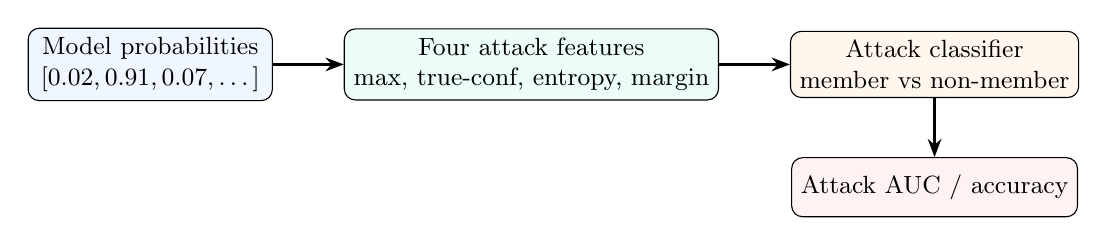
\begin{tikzpicture}[
  font=\small,
  box/.style={draw,rounded corners,align=center,minimum width=3.1cm,minimum height=0.75cm},
  arr/.style={-{Stealth},thick}
]
\node[box,fill=bluebox] (prob) {Model probabilities\\\(\left[0.02,0.91,0.07,\dots\right]\)};
\node[box,fill=greenbox,right=0.9cm of prob] (feat) {Four attack features\\max, true-conf, entropy, margin};
\node[box,fill=orangebox,right=0.9cm of feat] (clf) {Attack classifier\\member vs non-member};
\node[box,fill=redbox,below=0.75cm of clf] (metric) {Attack AUC / accuracy};
\draw[arr] (prob) -- (feat);
\draw[arr] (feat) -- (clf);
\draw[arr] (clf) -- (metric);
\end{tikzpicture}
\end{center}

\subsection{Confidence Attack}

\code{confidence_attack} stacks member features and non-member features, labels them 1/0, shuffles, trains logistic regression on half, and evaluates on half. It returns:
\[
(\text{confidence AUC},\ \text{confidence accuracy},\ \text{threshold AUC},\ \text{threshold accuracy})
\]
This attack is simple but powerful because models often assign higher confidence to training samples.

\subsection{Threshold Attack}

The threshold attack uses only true-label confidence \(p_{i,y_i}\). It computes ROC AUC from the raw confidence scores and an accuracy from median-threshold predictions.

\subsection{Shadow Attack}

\code{shadow_attack} trains an attacker on outputs from a shadow model:
\begin{enumerate}
  \item Train a shadow model on a separate split/synthetic draw.
  \item Label shadow train nodes as members and shadow test nodes as non-members.
  \item Train attack logistic regression on shadow features.
  \item Evaluate attack model on target-model member/non-member features.
\end{enumerate}

\subsection{LiRA Placeholder}

\file{lira_attack.py} currently contains:
\[
\code{return 0.5, 0.5}
\]
So LiRA values in results are chance-level placeholders unless that file is replaced with a real implementation. Any paper claim based on LiRA should not be made from this checkout as-is.

\subsection{Expected Calibration Error}

\code{calibration_error} bins samples by max confidence and sums:
\[
\text{ECE}=\sum_b \frac{|B_b|}{n}\left|\text{acc}(B_b)-\text{conf}(B_b)\right|.
\]
ECE is not an attack. It measures whether confidence values are honest. Poor calibration can correlate with higher leakage.

%==============================================================================
\section{The Single-Run Engine: \file{experiment.py}}
%==============================================================================

\file{experiment.py} is the heart of the project. Its main public function is \code{run_one}. It produces exactly one row in \file{all_results.csv}.

\subsection{High-Level Call Flow}

\begin{center}
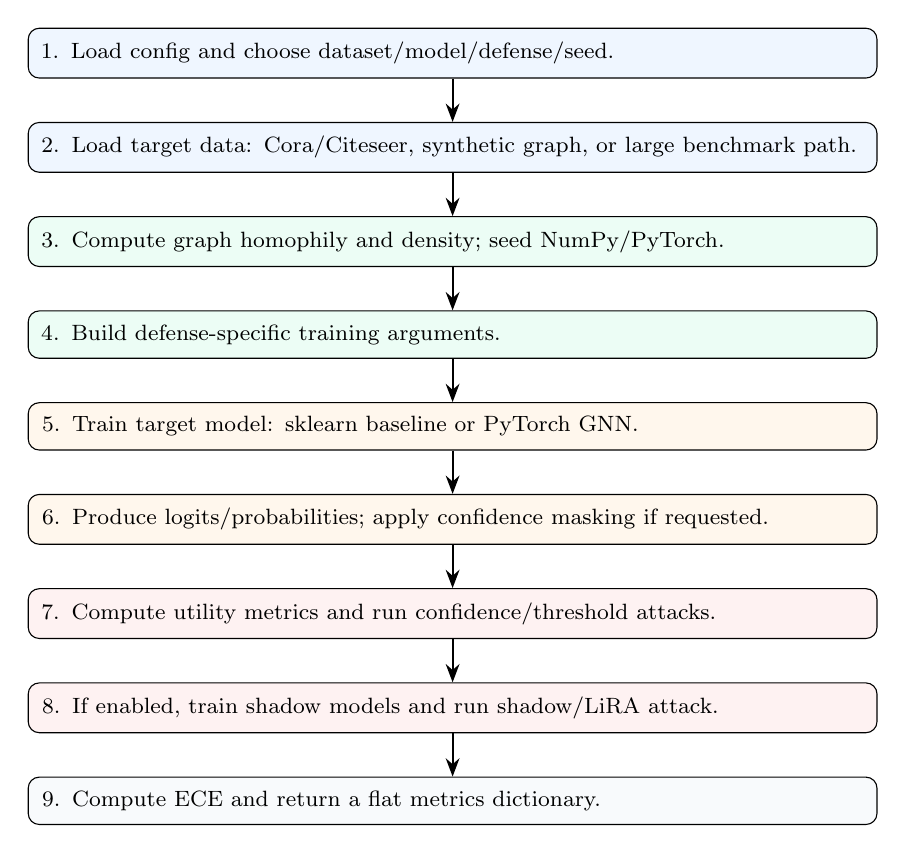
\begin{tikzpicture}[
  font=\footnotesize,
  node distance=0.55cm,
  procstep/.style={draw,rounded corners,align=left,text width=0.86\textwidth,inner sep=5pt},
  arr/.style={-{Stealth},thick}
]
\node[procstep,fill=bluebox] (s1) {1. Load config and choose dataset/model/defense/seed.};
\node[procstep,fill=bluebox,below=of s1] (s2) {2. Load target data: Cora/Citeseer, synthetic graph, or large benchmark path.};
\node[procstep,fill=greenbox,below=of s2] (s3) {3. Compute graph homophily and density; seed NumPy/PyTorch.};
\node[procstep,fill=greenbox,below=of s3] (s4) {4. Build defense-specific training arguments.};
\node[procstep,fill=orangebox,below=of s4] (s5) {5. Train target model: sklearn baseline or PyTorch GNN.};
\node[procstep,fill=orangebox,below=of s5] (s6) {6. Produce logits/probabilities; apply confidence masking if requested.};
\node[procstep,fill=redbox,below=of s6] (s7) {7. Compute utility metrics and run confidence/threshold attacks.};
\node[procstep,fill=redbox,below=of s7] (s8) {8. If enabled, train shadow models and run shadow/LiRA attack.};
\node[procstep,fill=graybox,below=of s8] (s9) {9. Compute ECE and return a flat metrics dictionary.};
\foreach \a/\b in {s1/s2,s2/s3,s3/s4,s4/s5,s5/s6,s6/s7,s7/s8,s8/s9}
  \draw[arr] (\a) -- (\b);
\end{tikzpicture}
\end{center}

\subsection{Dataset Dispatch}

\code{_load_target_data} uses dataset name rules:
\begin{itemize}
  \item \code{Cora}, \code{Citeseer}: load Planetoid then resplit.
  \item \code{synthetic_*_*}: parse the name into homophily and density.
  \item names in \code{MINIBATCH_DATASETS}: large-graph path, currently unreachable because the set is empty.
\end{itemize}

\subsection{Model Dispatch}

\begin{itemize}
  \item \code{GCN} and \code{GraphSAGE}: PyTorch model + \file{training.py}.
  \item \code{LogReg}: sklearn logistic regression.
  \item \code{MLP}: sklearn MLP classifier.
\end{itemize}

\subsection{Returned Metrics}

The row contains:
\begin{itemize}
  \item identifiers: dataset, model, defense, params, seed,
  \item graph stats: homophily, density,
  \item utility: test accuracy, macro F1, test AUROC,
  \item attack metrics: confidence, threshold, shadow, LiRA,
  \item calibration: ECE,
  \item privacy budget: DP epsilon if DP-SGD ran.
\end{itemize}

%==============================================================================
\section{Configuration System}
%==============================================================================

\subsection{Default Config}

\file{config.py} contains built-in defaults, but normally it reads YAML. The environment variable \code{PRIVACYGNN_CONFIG} can override the config path:
\[
\code{PRIVACYGNN_CONFIG=experiment_config_paper.yaml python run_final.py}
\]

\subsection{Grid Construction}

\code{get_experiment_list} loops:
\[
\text{datasets}\times\text{models}\times\text{defenses}\times\text{seeds}.
\]
It skips invalid combinations:
\begin{itemize}
  \item LogReg and MLP only run \code{none}.
  \item DP-SGD only applies to GCN/GraphSAGE.
  \item DP-SGD can be restricted to certain datasets.
\end{itemize}

\subsection{Current Result Grid}

The current \file{results/all_results.csv} contains:
\begin{itemize}
  \item 560 rows and 20 columns,
  \item 8 datasets: Cora, Citeseer, and six synthetic regimes,
  \item 4 models: LogReg, MLP, GCN, GraphSAGE,
  \item 6 defenses in the result table,
  \item 5 seeds: 42, 123, 456, 789, 1024.
\end{itemize}

%==============================================================================
\section{Main Runner and Output Files}
%==============================================================================

\subsection{\texttt{run\_final.py}}

\file{run_final.py} performs the production run:
\begin{enumerate}
  \item load config,
  \item ensure directories,
  \item build experiment list,
  \item loop over all combinations,
  \item call \code{run_one},
  \item periodically checkpoint partial results,
  \item write full results,
  \item aggregate summary,
  \item run significance tests,
  \item run bootstrap summary.
\end{enumerate}

\subsection{Output CSVs}

\begin{longtable}{@{}L{0.27\textwidth}L{0.14\textwidth}L{0.53\textwidth}@{}}
\toprule
\textbf{File} & \textbf{Shape} & \textbf{Meaning}\\
\midrule
\endhead
\file{results/all_results.csv} & 560 x 20 & One row per complete run. This is the raw experimental table.\\
\file{results/summary.csv} & 112 x 16 & Grouped by dataset/model/defense, with means/stds.\\
\file{results/significance.csv} & 80 x 7 & Paired t-tests for confidence attack AUC, defense vs no defense.\\
\file{results/significance_lira.csv} & 80 x 7 & Same structure for LiRA AUC, but LiRA is placeholder here.\\
\file{results/summary_bootstrap.csv} & 448 x 9 & Bootstrap confidence intervals over seeds for metrics.\\
\file{results/all_results.partial.csv} & varies & Checkpoint written every 50 completed rows during long runs.\\
\bottomrule
\end{longtable}

%==============================================================================
\section{Statistics Layer}
%==============================================================================

\subsection{Paired t-tests}

\file{stats_utils.py} compares each defense against \code{none}, paired by seed within the same dataset/model group. This is important because paired comparisons reduce noise from random splits.

\[
d_s = \text{AUC}_{\text{defense},s}-\text{AUC}_{\text{none},s}
\]
Then SciPy's paired t-test evaluates whether the mean difference is distinguishable from zero.

\subsection{Bootstrap Confidence Intervals}

The bootstrap function resamples seeds with replacement inside each dataset/model/defense group. It estimates uncertainty for metric means and writes percentile intervals:
\[
[\text{quantile}_{\alpha/2},\ \text{quantile}_{1-\alpha/2}].
\]
This is separate from p-values.

\subsection{How to Interpret Statistics Carefully}

The project uses only five seeds in the paper config/current results. That is useful but not huge. Treat p-values as exploratory evidence, not final proof. Bootstrap CIs are better for communicating uncertainty visually.

%==============================================================================
\section{Visualization Scripts}
%==============================================================================

\subsection{\texttt{generate\_figures.py}: Publication Figures}

This script reads \file{all_results.csv} and produces six paper-oriented figures:
\begin{enumerate}
  \item attack AUC vs model on Cora/Citeseer,
  \item privacy-utility tradeoff,
  \item leakage vs homophily,
  \item defense effectiveness,
  \item leakage vs density,
  \item comprehensive heatmap.
\end{enumerate}
It includes checks for missing Cora/Citeseer rows and falls back for Figure 2 if Cora GNN results are absent.

\subsection{\texttt{generate\_basic\_figures.py}}

This script reads \file{summary.csv} and focuses on synthetic summaries:
\begin{itemize}
  \item grouped bar chart of attack AUC by model,
  \item GCN-only leakage by setting,
  \item GCN defenses on low-homophily medium setting,
  \item heatmap of model by setting.
\end{itemize}

\subsection{\texttt{generate\_final\_visuals.py}}

This script creates polished presentation graphics in \file{../Final Visuals}. It emphasizes:
\begin{itemize}
  \item worst-case low-homophily sparse setting,
  \item GCN vs GraphSAGE trajectories,
  \item defense comparison,
  \item privacy-utility point cloud,
  \item attack-AUC matrix.
\end{itemize}

\subsection{\texttt{generate\_poster\_visuals.py}}

This is the most extensive visual suite. It creates 11 poster-ready outputs:
\begin{itemize}
  \item study pipeline,
  \item leakage heatmap,
  \item privacy-utility landscape,
  \item defense delta heatmap,
  \item defense ranking,
  \item attack family comparison,
  \item homophily/density effects,
  \item calibration vs leakage,
  \item significance heatmap,
  \item regime small multiples,
  \item summary table.
\end{itemize}

\subsection{\texttt{fix\_figures.py}}

This script regenerates improved versions of Figure 2 and Figure 4. It uses \code{adjustText} to reduce label overlap. It writes PNG and PDF versions.

%==============================================================================
\section{Paper, Poster, and Slide Assets}
%==============================================================================

\subsection{\texttt{paper/ieee\_privacy\_gnn.tex}}

This is the main IEEE-style manuscript source. Use it for academic writing, but keep it synchronized with current code and result files.

\subsection{\texttt{paper/build\_manuscript.py}}

This script uses ReportLab to create a static PDF manuscript. It includes narrative text, tables, and references directly in Python. Because it is hand-written, it can drift from the live code. For example, code defaults in the actual pipeline use 50 epochs and 50/50 splits for many paths, while manuscript text may describe other protocol settings. Always verify claims against \file{experiment_config_paper.yaml}, \file{run_final.py}, and \file{all_results.csv}.

\subsection{\texttt{paper/build\_project\_slides.py}}

This script uses \code{python-pptx} to create a clean slide deck. It defines a small design system (colors, fonts, footer) and adds slides explaining the study, datasets, models, attacks, defenses, takeaways, and limitations.

%==============================================================================
\section{How the Methods Differ}
%==============================================================================

\begin{longtable}{@{}L{0.18\textwidth}L{0.24\textwidth}L{0.52\textwidth}@{}}
\toprule
\textbf{Method family} & \textbf{Specific methods} & \textbf{Key difference}\\
\midrule
\endhead
Models & LogReg, MLP, GCN, GraphSAGE & Baselines ignore graph edges; GNNs use neighborhood aggregation.\\
Graph regimes & High/low homophily, sparse/medium/dense & Tests whether structure affects privacy leakage.\\
Defenses & DropEdge, smoothing, early stop, masking, sparsification & Some change training, some change graph, one changes output probabilities.\\
Attacks & Confidence, threshold, shadow, LiRA placeholder & Confidence/shadow learn an attack classifier; threshold is direct; LiRA is not implemented.\\
Statistics & t-tests, bootstrap CIs & t-tests compare defense vs none; bootstrap estimates uncertainty over seeds.\\
Visuals & Basic, paper, final, poster & Same data, different presentation goals and levels of polish.\\
\bottomrule
\end{longtable}

%==============================================================================
\section{Testing and Validation Status}
%==============================================================================

\subsection{What Exists}

There is no dedicated automated unit-test suite in the current repository. No \file{tests/} directory, \file{test_*.py}, or pytest configuration was found in the project survey.

The project instead validates behavior through:
\begin{itemize}
  \item reproducible config-driven execution,
  \item deterministic seeds,
  \item CSV outputs for every run,
  \item aggregation and paired comparisons,
  \item bootstrap uncertainty,
  \item figure generation from saved results,
  \item manual inspection through \file{RESULTS_ANALYSIS.md}.
\end{itemize}

\subsection{Recommended Tests to Add}

If you want engineering-grade confidence, add:
\begin{itemize}
  \item unit tests for \code{make_synthetic}: node count, feature shape, mask sizes, density range, homophily trend;
  \item unit tests for \code{extract_features}: output shape and known probability cases;
  \item unit tests for \code{confidence_attack}: random synthetic probabilities give AUC near 0.5;
  \item smoke test for \code{run_one} on one tiny synthetic graph;
  \item config-grid test ensuring LogReg/MLP skip graph-only defenses;
  \item regression test ensuring \code{summary.csv} columns are stable;
  \item figure-generation smoke test using a small fake CSV.
\end{itemize}

%==============================================================================
\section{Known Limitations and Technical Debt}
%==============================================================================

\begin{longtable}{@{}L{0.24\textwidth}L{0.70\textwidth}@{}}
\toprule
\textbf{Limitation} & \textbf{Technical meaning}\\
\midrule
\endhead
LiRA placeholder & \file{lira_attack.py} returns 0.5 metrics. It is not a real LiRA implementation.\\
Large graphs stubbed & \file{ogb_loader.py} has an empty dataset set; \file{graph_minibatch.py} raises \code{NotImplementedError}.\\
DP-SGD path inactive & Config includes DP-SGD fields, but the implementation depends on stubbed minibatch DP training.\\
No automated tests & The project is reproducible but not unit-tested.\\
Some generated paper text may drift & ReportLab manuscript script is static text and should be checked against live result files.\\
Attack assumptions & Attacks use true labels in feature extraction. This is common in some MIA evaluations but should be stated clearly.\\
Only node-level classification & Link-level, graph-level, subgraph-level, and inductive privacy are not fully studied.\\
\bottomrule
\end{longtable}

%==============================================================================
\section{How to Learn the Codebase Efficiently}
%==============================================================================

\begin{enumerate}
  \item Start with \file{experiment_config_paper.yaml}; understand the grid.
  \item Read \file{run_final.py}; understand how rows are created and aggregated.
  \item Read \code{run_one} in \file{experiment.py}; this is the core control flow.
  \item Read \file{data.py}; understand synthetic graph generation and masks.
  \item Read \file{models.py} and \file{training.py}; understand GCN/GraphSAGE and defenses.
  \item Read \file{attacks.py}; understand the four attack features and attack AUC.
  \item Open \file{results/all_results.csv}; identify one row and trace how it was produced.
  \item Open \file{summary.csv}; connect raw rows to means/stds.
  \item Read \file{RESULTS_ANALYSIS.md}; compare interpretations against the CSVs.
  \item Study the figure scripts last; they are presentation layers over saved results.
\end{enumerate}

%==============================================================================
\section{Command Cheat Sheet}
%==============================================================================

\begin{verbatim}
# Install dependencies
cd privacy-gnn
pip install -r requirements.txt

# Run default configured grid
python run_final.py

# Run paper-aligned grid
PRIVACYGNN_CONFIG=experiment_config_paper.yaml python run_final.py

# Generate publication figures
python generate_figures.py

# Generate basic synthetic figures
python generate_basic_figures.py

# Generate final presentation visuals
python generate_final_visuals.py

# Generate poster visual suite
python generate_poster_visuals.py

# Build manuscript from ReportLab script
python paper/build_manuscript.py

# Build slide deck
python paper/build_project_slides.py
\end{verbatim}

%==============================================================================
\section{Final Mental Model}
%==============================================================================

If you remember only one thing, remember this:

\begin{quote}
\textbf{PrivacyGNN is a controlled experiment engine. The config defines a grid. \file{run_final.py} executes the grid. \file{experiment.py} creates one metrics row. \file{attacks.py} turns prediction confidence into membership-inference scores. The results CSVs are the source of truth for all figures and claims.}
\end{quote}

The intellectual contribution is not merely ``training a GNN.'' It is the systematic comparison of models, graph structures, defenses, and attacks under reproducible seeds, with graph structure measured and controlled.

\end{document}
